\chapter{Infrared spectra}
\label{chap:irSpectra}

In this chapter we present some general observations and discuss with more detail the infrared-active exctitations.
We start with section \ref{sec:classification} describing the general nature of the different excitations. 
In section \ref{sec:irSpectra} we analyze some features that should be present in the infrared spectra followed, in section \ref{sec:irIsotopicShifts}, by a description of the effects that the isotopic $^{16}$O$\rightarrow ^{18}$O substitution has in the spectra. 
Finally we conclude in section \ref{sec:irPhononProj} with some observations about the projections into the phonon coordinates of these infrared-active states.

\section{Classification of the excitations}
\label{sec:classification}

As previously noted in section \ref{sec:hamiltonian-and-basis}, only for zero charge-lattice couplings the eigenstates of the many-body Hamiltonian (\ref{eq:full-hamiltonian}) can be described as a direct product of an electronic and a phononic state, that is, eigenstates of the full hamiltonian $H$ are products of eigenstates of $H_{el}$ and $H_{ph}$ respectively.
In this uncoupled scenario the phonon number opreators $b_Rb^\dagger_R$ and $b_{ir}b^\dagger_{ir}$ have integer values with zero dispersion.
Increasing the value of the coupling parameters produces eigenstates with different mean phonon values and some finite dispersion producing eigenstates that can not be separated as a product of phononic and electronic states.
However, the deviation from this behaviour is smooth in the coupling parameter $\lambda_{ir}$.
That is, a hamiltonian with a small $\lambda_{ir}$ value will have only slighty different eigenstates from the uncoupled hamiltonian.
These slightly mixed eigenstates in the small couping regime can be thought of as largely \textit{phononic} or \textit{electronic} in nature.
For larger coupling values the eigenstates are very different from their uncoupled counterparts.
As an illustration of this we show, in figure \ref{fig:electr-proj}, the first electronic excitation for different $\lambda_{ir}$ values, $\psi_{el}(\lambda_{ir})$ projected unto the first electronic state on the uncoupled system, $\psi_{el}(\lambda_{ir}=0)$.
From this projection we can see that for small coupling values $\psi_{el}$ remains largely unchanged, that is, it remains \textit{electronic} in nature.
In the middle coupling regime the change is the strongest with the projection approaching asymptotically to zero at large couplings.
The vertical line in \ref{fig:electr-proj} at $\lambda_{ir}=0.1263$ eV, as discussed in section \ref{sec:grd-phonon-proj}, represents the $\lambda_{ir}$ value that reproduces the experimentally observed cluster distortion of 0.13 \AA.
At this coupling value the electronic eigenstate has a projection unto its uncoupled counterpart near 0.75 which indicates that, although it has been somewhat changed, it remains mostly \textit{electronic} in nature.
Similar observations can be made for the rest of the excitations in this model.
For this reason even though the eigenstates, for finite charge-lattice couplings, are not strictly electronic or phononic we will continue to refer to them as such since that interpretation remains useful in the regime of interest to us.
Given the possibility of making such a distinction for the different excitations we will discuss \textit{phononic} and \textit{electronic} excitations separatedly in this and the next chapters respectively. 
%
\begin{figure}[ht]
  \centering
  % GNUPLOT: LaTeX picture with Postscript
\begingroup
  \makeatletter
  \providecommand\color[2][]{%
    \GenericError{(gnuplot) \space\space\space\@spaces}{%
      Package color not loaded in conjunction with
      terminal option `colourtext'%
    }{See the gnuplot documentation for explanation.%
    }{Either use 'blacktext' in gnuplot or load the package
      color.sty in LaTeX.}%
    \renewcommand\color[2][]{}%
  }%
  \providecommand\includegraphics[2][]{%
    \GenericError{(gnuplot) \space\space\space\@spaces}{%
      Package graphicx or graphics not loaded%
    }{See the gnuplot documentation for explanation.%
    }{The gnuplot epslatex terminal needs graphicx.sty or graphics.sty.}%
    \renewcommand\includegraphics[2][]{}%
  }%
  \providecommand\rotatebox[2]{#2}%
  \@ifundefined{ifGPcolor}{%
    \newif\ifGPcolor
    \GPcolortrue
  }{}%
  \@ifundefined{ifGPblacktext}{%
    \newif\ifGPblacktext
    \GPblacktextfalse
  }{}%
  % define a \g@addto@macro without @ in the name:
  \let\gplgaddtomacro\g@addto@macro
  % define empty templates for all commands taking text:
  \gdef\gplbacktext{}%
  \gdef\gplfronttext{}%
  \makeatother
  \ifGPblacktext
    % no textcolor at all
    \def\colorrgb#1{}%
    \def\colorgray#1{}%
  \else
    % gray or color?
    \ifGPcolor
      \def\colorrgb#1{\color[rgb]{#1}}%
      \def\colorgray#1{\color[gray]{#1}}%
      \expandafter\def\csname LTw\endcsname{\color{white}}%
      \expandafter\def\csname LTb\endcsname{\color{black}}%
      \expandafter\def\csname LTa\endcsname{\color{black}}%
      \expandafter\def\csname LT0\endcsname{\color[rgb]{1,0,0}}%
      \expandafter\def\csname LT1\endcsname{\color[rgb]{0,1,0}}%
      \expandafter\def\csname LT2\endcsname{\color[rgb]{0,0,1}}%
      \expandafter\def\csname LT3\endcsname{\color[rgb]{1,0,1}}%
      \expandafter\def\csname LT4\endcsname{\color[rgb]{0,1,1}}%
      \expandafter\def\csname LT5\endcsname{\color[rgb]{1,1,0}}%
      \expandafter\def\csname LT6\endcsname{\color[rgb]{0,0,0}}%
      \expandafter\def\csname LT7\endcsname{\color[rgb]{1,0.3,0}}%
      \expandafter\def\csname LT8\endcsname{\color[rgb]{0.5,0.5,0.5}}%
    \else
      % gray
      \def\colorrgb#1{\color{black}}%
      \def\colorgray#1{\color[gray]{#1}}%
      \expandafter\def\csname LTw\endcsname{\color{white}}%
      \expandafter\def\csname LTb\endcsname{\color{black}}%
      \expandafter\def\csname LTa\endcsname{\color{black}}%
      \expandafter\def\csname LT0\endcsname{\color{black}}%
      \expandafter\def\csname LT1\endcsname{\color{black}}%
      \expandafter\def\csname LT2\endcsname{\color{black}}%
      \expandafter\def\csname LT3\endcsname{\color{black}}%
      \expandafter\def\csname LT4\endcsname{\color{black}}%
      \expandafter\def\csname LT5\endcsname{\color{black}}%
      \expandafter\def\csname LT6\endcsname{\color{black}}%
      \expandafter\def\csname LT7\endcsname{\color{black}}%
      \expandafter\def\csname LT8\endcsname{\color{black}}%
    \fi
  \fi
  \setlength{\unitlength}{0.0500bp}%
  \begin{picture}(6802.00,3968.00)%
    \gplgaddtomacro\gplbacktext{%
      \colorrgb{0.31,0.31,0.31}%
      \put(1078,751){\makebox(0,0)[r]{\strut{}\scriptsize 0}}%
      \colorrgb{0.31,0.31,0.31}%
      \put(1078,1313){\makebox(0,0)[r]{\strut{}\scriptsize 0.2}}%
      \colorrgb{0.31,0.31,0.31}%
      \put(1078,1876){\makebox(0,0)[r]{\strut{}\scriptsize 0.4}}%
      \colorrgb{0.31,0.31,0.31}%
      \put(1078,2438){\makebox(0,0)[r]{\strut{}\scriptsize 0.6}}%
      \colorrgb{0.31,0.31,0.31}%
      \put(1078,3000){\makebox(0,0)[r]{\strut{}\scriptsize 0.8}}%
      \colorrgb{0.31,0.31,0.31}%
      \put(1078,3562){\makebox(0,0)[r]{\strut{}\scriptsize 1}}%
      \colorrgb{0.31,0.31,0.31}%
      \put(1257,484){\makebox(0,0){\strut{}\scriptsize 0}}%
      \colorrgb{0.31,0.31,0.31}%
      \put(1669,484){\makebox(0,0){\strut{}\scriptsize 0.02}}%
      \colorrgb{0.31,0.31,0.31}%
      \put(2081,484){\makebox(0,0){\strut{}\scriptsize 0.04}}%
      \colorrgb{0.31,0.31,0.31}%
      \put(2493,484){\makebox(0,0){\strut{}\scriptsize 0.06}}%
      \colorrgb{0.31,0.31,0.31}%
      \put(2904,484){\makebox(0,0){\strut{}\scriptsize 0.08}}%
      \colorrgb{0.31,0.31,0.31}%
      \put(3316,484){\makebox(0,0){\strut{}\scriptsize 0.1}}%
      \colorrgb{0.31,0.31,0.31}%
      \put(3728,484){\makebox(0,0){\strut{}\scriptsize 0.12}}%
      \colorrgb{0.31,0.31,0.31}%
      \put(4140,484){\makebox(0,0){\strut{}\scriptsize 0.14}}%
      \colorrgb{0.31,0.31,0.31}%
      \put(4552,484){\makebox(0,0){\strut{}\scriptsize 0.16}}%
      \colorrgb{0.31,0.31,0.31}%
      \put(4964,484){\makebox(0,0){\strut{}\scriptsize 0.18}}%
      \colorrgb{0.31,0.31,0.31}%
      \put(5375,484){\makebox(0,0){\strut{}\scriptsize 0.2}}%
      \colorrgb{0.31,0.31,0.31}%
      \put(5787,484){\makebox(0,0){\strut{}\scriptsize 0.22}}%
      \colorrgb{0.31,0.31,0.31}%
      \put(6199,484){\makebox(0,0){\strut{}\scriptsize 0.24}}%
      \csname LTb\endcsname%
      \put(176,2227){\rotatebox{-270}{\makebox(0,0){\strut{}$\left|\braket{\psi_{el} (\lambda_{ir}=0)}{\psi_{el} (\lambda_{ir})}\right|$}}}%
      \put(3831,154){\makebox(0,0){\strut{}$\lambda_{ir}$ (eV)}}%
      \put(3934,3467){\makebox(0,0)[l]{\strut{}\scriptsize$\lambda_{ir}=0.1263$}}%
    }%
    \gplgaddtomacro\gplfronttext{%
    }%
    \gplbacktext
    \put(0,0){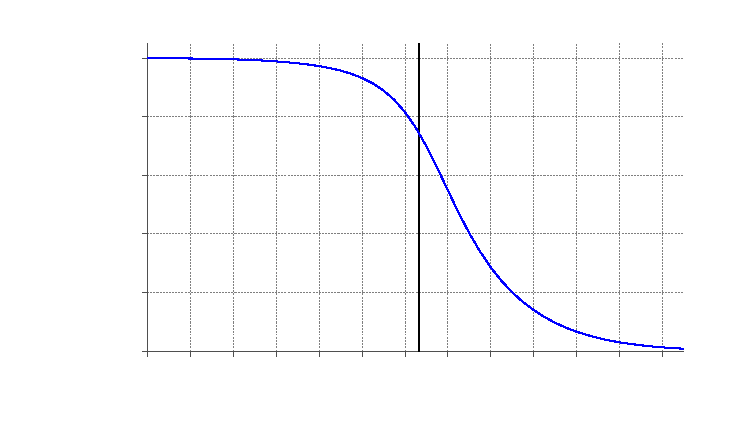
\includegraphics{images/electrProj}}%
    \gplfronttext
  \end{picture}%
\endgroup

  \caption[Projection of the first \textit{electronic} state with itself at $\lambda_{ir}=0$.]
  {Projection of the first \textit{electronic} state with itself at $\lambda_{ir}=0$.
    The vertical line denotes the experimentally relevant value $\lambda_{ir}=0.1263$ eV.}
  \label{fig:electr-proj}
\end{figure}

Since we are setting the charge-lattice coupling parameter to the symmetrical (Raman) vibrational mode ($\lambda_R$) as zero and these excitations are unchanged by an increase in $\lambda_{ir}$, all eigenstates will have a definite eigenvalue for the Raman number operator $b_R^\dagger b_R$. 
An excitation which, at $\lambda_{ir}=0$, has an eigenvalue of zero for the infrared number operator $b_{ir}^\dagger b_{ir}$ and for the electronic part of the hamiltonian $H_{el}$ (i.e. it is a pure \textit{Raman} excitation with no other components) will remain completely unchanged with a variation in $\lambda_{ir}$.
We will omit any further discussion about these excitations and ignore them for the rest of this thesis. 


\section{Infrared spectra}
\label{sec:irSpectra}

The Peierls-Hubbard model (\ref{eq:full-hamiltonian}) applied to the O(4)-Cu(1)-O(4) cluster in YBa$_2$Cu$_3$O$_7$ should be able to predict some features of the c-axis infrared spectra by looking at its infrared-active excitations.
An excitation is infrared-active only when it has an opposite parity to the ground state.
At $\lambda_{ir}=0$ the excitations are harmonic and have an opposite parity if the number of infrared phonons is even or odd, this means that only the excitations with an odd number of infrared phonons are infrared-active.
Furthermore, since the coupling $\lambda_{ir}$ can be varied smoothly, the hamiltonian eigenstates will not change parity as a function of $\lambda_{ir}$ so it can be concluded that the infrared-active excitations, for any $\lambda_{ir}$, will be those that, at $\lambda_{ir}=0$, have an \textit{odd} number of phonons.

Figure \ref{fig:irSpectra} shows the frequencies of the infrared excitations for a representative range of $\lambda_{ir}$ values.
For $\lambda_{ir}=0$ we have excitations corresponding to the phononic part of the hamiltonian alone.
As can be observed, the behaviour of each excitation depends on the number of infrared phonons at zero coupling.
The number of Raman phonons only displaces the excitation in multiples of $\omega_R=500$ cm$^{-1}$.
That is, all the red lines in Fig.\ \ref{fig:irSpectra} correspond to one infrared phonon and, in ascending order, have zero, one and two Raman phonons.
This is similarly true for the excitations with two (green lines) and three (blue lines) infrared phonons.
Notice that the excitations with two infrared phonons are not infrared-active since they have the same symmetry as the ground state.
%
\begin{figure}[ht]
  \centering
  % GNUPLOT: LaTeX picture with Postscript
\begingroup
  \makeatletter
  \providecommand\color[2][]{%
    \GenericError{(gnuplot) \space\space\space\@spaces}{%
      Package color not loaded in conjunction with
      terminal option `colourtext'%
    }{See the gnuplot documentation for explanation.%
    }{Either use 'blacktext' in gnuplot or load the package
      color.sty in LaTeX.}%
    \renewcommand\color[2][]{}%
  }%
  \providecommand\includegraphics[2][]{%
    \GenericError{(gnuplot) \space\space\space\@spaces}{%
      Package graphicx or graphics not loaded%
    }{See the gnuplot documentation for explanation.%
    }{The gnuplot epslatex terminal needs graphicx.sty or graphics.sty.}%
    \renewcommand\includegraphics[2][]{}%
  }%
  \providecommand\rotatebox[2]{#2}%
  \@ifundefined{ifGPcolor}{%
    \newif\ifGPcolor
    \GPcolortrue
  }{}%
  \@ifundefined{ifGPblacktext}{%
    \newif\ifGPblacktext
    \GPblacktextfalse
  }{}%
  % define a \g@addto@macro without @ in the name:
  \let\gplgaddtomacro\g@addto@macro
  % define empty templates for all commands taking text:
  \gdef\gplbacktext{}%
  \gdef\gplfronttext{}%
  \makeatother
  \ifGPblacktext
    % no textcolor at all
    \def\colorrgb#1{}%
    \def\colorgray#1{}%
  \else
    % gray or color?
    \ifGPcolor
      \def\colorrgb#1{\color[rgb]{#1}}%
      \def\colorgray#1{\color[gray]{#1}}%
      \expandafter\def\csname LTw\endcsname{\color{white}}%
      \expandafter\def\csname LTb\endcsname{\color{black}}%
      \expandafter\def\csname LTa\endcsname{\color{black}}%
      \expandafter\def\csname LT0\endcsname{\color[rgb]{1,0,0}}%
      \expandafter\def\csname LT1\endcsname{\color[rgb]{0,1,0}}%
      \expandafter\def\csname LT2\endcsname{\color[rgb]{0,0,1}}%
      \expandafter\def\csname LT3\endcsname{\color[rgb]{1,0,1}}%
      \expandafter\def\csname LT4\endcsname{\color[rgb]{0,1,1}}%
      \expandafter\def\csname LT5\endcsname{\color[rgb]{1,1,0}}%
      \expandafter\def\csname LT6\endcsname{\color[rgb]{0,0,0}}%
      \expandafter\def\csname LT7\endcsname{\color[rgb]{1,0.3,0}}%
      \expandafter\def\csname LT8\endcsname{\color[rgb]{0.5,0.5,0.5}}%
    \else
      % gray
      \def\colorrgb#1{\color{black}}%
      \def\colorgray#1{\color[gray]{#1}}%
      \expandafter\def\csname LTw\endcsname{\color{white}}%
      \expandafter\def\csname LTb\endcsname{\color{black}}%
      \expandafter\def\csname LTa\endcsname{\color{black}}%
      \expandafter\def\csname LT0\endcsname{\color{black}}%
      \expandafter\def\csname LT1\endcsname{\color{black}}%
      \expandafter\def\csname LT2\endcsname{\color{black}}%
      \expandafter\def\csname LT3\endcsname{\color{black}}%
      \expandafter\def\csname LT4\endcsname{\color{black}}%
      \expandafter\def\csname LT5\endcsname{\color{black}}%
      \expandafter\def\csname LT6\endcsname{\color{black}}%
      \expandafter\def\csname LT7\endcsname{\color{black}}%
      \expandafter\def\csname LT8\endcsname{\color{black}}%
    \fi
  \fi
  \setlength{\unitlength}{0.0500bp}%
  \begin{picture}(6802.00,4534.00)%
    \gplgaddtomacro\gplbacktext{%
      \colorrgb{0.31,0.31,0.31}%
      \put(990,751){\makebox(0,0)[r]{\strut{}\scriptsize 0}}%
      \colorrgb{0.31,0.31,0.31}%
      \put(990,1191){\makebox(0,0)[r]{\strut{}\scriptsize 250}}%
      \colorrgb{0.31,0.31,0.31}%
      \put(990,1631){\makebox(0,0)[r]{\strut{}\scriptsize 500}}%
      \colorrgb{0.31,0.31,0.31}%
      \put(990,2070){\makebox(0,0)[r]{\strut{}\scriptsize 750}}%
      \colorrgb{0.31,0.31,0.31}%
      \put(990,2510){\makebox(0,0)[r]{\strut{}\scriptsize 1000}}%
      \colorrgb{0.31,0.31,0.31}%
      \put(990,2950){\makebox(0,0)[r]{\strut{}\scriptsize 1250}}%
      \colorrgb{0.31,0.31,0.31}%
      \put(990,3390){\makebox(0,0)[r]{\strut{}\scriptsize 1500}}%
      \colorrgb{0.31,0.31,0.31}%
      \put(990,3829){\makebox(0,0)[r]{\strut{}\scriptsize 1750}}%
      \colorrgb{0.31,0.31,0.31}%
      \put(990,4269){\makebox(0,0)[r]{\strut{}\scriptsize 2000}}%
      \colorrgb{0.31,0.31,0.31}%
      \put(1169,484){\makebox(0,0){\strut{}\scriptsize 0}}%
      \colorrgb{0.31,0.31,0.31}%
      \put(1588,484){\makebox(0,0){\strut{}\scriptsize 0.02}}%
      \colorrgb{0.31,0.31,0.31}%
      \put(2007,484){\makebox(0,0){\strut{}\scriptsize 0.04}}%
      \colorrgb{0.31,0.31,0.31}%
      \put(2426,484){\makebox(0,0){\strut{}\scriptsize 0.06}}%
      \colorrgb{0.31,0.31,0.31}%
      \put(2845,484){\makebox(0,0){\strut{}\scriptsize 0.08}}%
      \colorrgb{0.31,0.31,0.31}%
      \put(3263,484){\makebox(0,0){\strut{}\scriptsize 0.1}}%
      \colorrgb{0.31,0.31,0.31}%
      \put(3682,484){\makebox(0,0){\strut{}\scriptsize 0.12}}%
      \colorrgb{0.31,0.31,0.31}%
      \put(4101,484){\makebox(0,0){\strut{}\scriptsize 0.14}}%
      \colorrgb{0.31,0.31,0.31}%
      \put(4520,484){\makebox(0,0){\strut{}\scriptsize 0.16}}%
      \colorrgb{0.31,0.31,0.31}%
      \put(4939,484){\makebox(0,0){\strut{}\scriptsize 0.18}}%
      \colorrgb{0.31,0.31,0.31}%
      \put(5358,484){\makebox(0,0){\strut{}\scriptsize 0.2}}%
      \colorrgb{0.31,0.31,0.31}%
      \put(5777,484){\makebox(0,0){\strut{}\scriptsize 0.22}}%
      \colorrgb{0.31,0.31,0.31}%
      \put(6196,484){\makebox(0,0){\strut{}\scriptsize 0.24}}%
      \csname LTb\endcsname%
      \put(352,2510){\rotatebox{-270}{\makebox(0,0){\strut{}$\omega_i$ (cm$^{-1}$)}}}%
      \put(3787,154){\makebox(0,0){\strut{}$\lambda_{ir}$ (eV)}}%
      \put(3892,3988){\makebox(0,0)[l]{\strut{}\scriptsize$\lambda_{ir}=0.1263$}}%
    }%
    \gplgaddtomacro\gplfronttext{%
    }%
    \gplbacktext
    \put(0,0){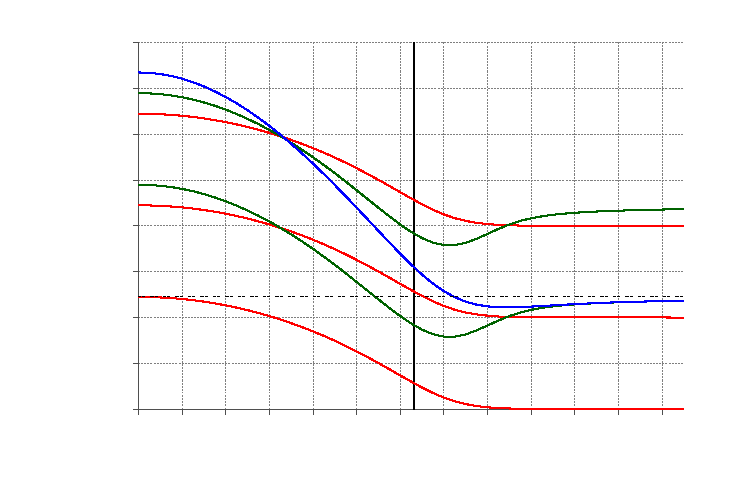
\includegraphics{images/irSpectra}}%
    \gplfronttext
  \end{picture}%
\endgroup

  \caption[Infrared-active excitations as a function of electron-lattice coupling.]
  {Infrared-active excitations as a function of electron-lattice coupling.
  The red, green and blue lines denote excitations which, initially, have one, two and three infrared phonons respectively.
  The horizontal dashed line is placed at the first infared-active excitation $\omega_i=612.4$ cm$^{-1}$ as a guide to the eye.}
  \label{fig:irSpectra}
\end{figure}

All the infrared excitations reach a lower energy asymptotically at large $\lambda_{ir}$ but only the state excitations with two infrared phonons have a minimum.
The excitations with one infrared phonon decrease in energy converging to the Raman energies ($0,\omega_R,2\omega_R\ldots$).
However the excitations with two and three infrared phonons converge to the infrared energies ($\omega_{ir},2\omega_{ir},3\omega_{ir}\ldots$).
This recovery of an harmonic behaviour at large $\lambda_{ir}$ is similiar to what was discussed in section \ref{sec:grd-phonon-proj} for the ground and first excited states which can be interpreted as a recovery of the harmonic behaviour but with a displaced equilibrium position.

It is interesting to notice that the infrared spectra at $\lambda_{ir}=0$ eV and at the relevant coupling, $\lambda_{ir}=0.1263$ eV, are very similar albeit with some noticeable differences.
The peak centered at 612.4 cm$^{-1}$ seems to be slightly shifted to 641.4 cm$^{-1}$ with an asymetry produced by the excitation with three infrared phonons at 774.2 cm$^{-1}$ \cite{MustredeLeon1992,Salkola1994}.
It should be noted that calculations using a rigid double-well potential for the O(4)-Cu(1)-O(4) cluster are unable to produce this asymmetry.
Also in the $\lambda_{ir}=0.1263$ eV case there is an aditional excitation at 142.4 cm$^{-1}$ which has not yet been observed since other absorption processes in this range, e. g. a large Drude contribution in the D. C. conductivity, make its detection difficult.

\section{Isotopic shifts}
\label{sec:irIsotopicShifts}

We also calculated the infrared spectra change under the O$^{16}\rightarrow$O$^{18}$ isotopic substitution and computed the corresponding isotopic shift, as defined by (\ref{eq:isot-shift-def-exc}), for each excitation.
In the top panel of Figure \ref{fig:irIsot} we show the isotopic shift for the first infrare-active excitation and in the bottom panel the isotopic shifts for the excitations with two (red line) and three (blue line) infrared phonons as well as the state with one infrared plus one Raman phonon (red line).

As expected, all isotopic shifts start at the harmonic value which is 3.75\% for the pure infrared excitations and 4.65\% for the excitation with one infrared plus one Raman phonons.
For large $\lambda_{ir}$ values the isotopic shifts of the infrared excitations with two and three phonons return asymptotically to the infrared harmonic value of 3.75\% but the isotopic shift of the excitation with one infrared plus one Raman phonons converges to the Raman value of 5.75\%.
This behaviour for large $\lambda_{ir}$ is a consecuense of these excitations converging to either $\omega_{ir}$ or $\omega_R$, as pointed out earlier.
There is some variation of the isotopic shifts in the intermediate coupling regime but they always remain positive.
It is interesting to notice that isotopic shift of the excitations with 3 infrared phonons and 1 infrared plus 1 Raman phonon have a minimum very close to the relevant coupling $\lambda_{ir}=0.1263$ eV.
%
\begin{figure}[ht]
  \centering
  % GNUPLOT: LaTeX picture with Postscript
\begingroup
  \makeatletter
  \providecommand\color[2][]{%
    \GenericError{(gnuplot) \space\space\space\@spaces}{%
      Package color not loaded in conjunction with
      terminal option `colourtext'%
    }{See the gnuplot documentation for explanation.%
    }{Either use 'blacktext' in gnuplot or load the package
      color.sty in LaTeX.}%
    \renewcommand\color[2][]{}%
  }%
  \providecommand\includegraphics[2][]{%
    \GenericError{(gnuplot) \space\space\space\@spaces}{%
      Package graphicx or graphics not loaded%
    }{See the gnuplot documentation for explanation.%
    }{The gnuplot epslatex terminal needs graphicx.sty or graphics.sty.}%
    \renewcommand\includegraphics[2][]{}%
  }%
  \providecommand\rotatebox[2]{#2}%
  \@ifundefined{ifGPcolor}{%
    \newif\ifGPcolor
    \GPcolortrue
  }{}%
  \@ifundefined{ifGPblacktext}{%
    \newif\ifGPblacktext
    \GPblacktextfalse
  }{}%
  % define a \g@addto@macro without @ in the name:
  \let\gplgaddtomacro\g@addto@macro
  % define empty templates for all commands taking text:
  \gdef\gplbacktext{}%
  \gdef\gplfronttext{}%
  \makeatother
  \ifGPblacktext
    % no textcolor at all
    \def\colorrgb#1{}%
    \def\colorgray#1{}%
  \else
    % gray or color?
    \ifGPcolor
      \def\colorrgb#1{\color[rgb]{#1}}%
      \def\colorgray#1{\color[gray]{#1}}%
      \expandafter\def\csname LTw\endcsname{\color{white}}%
      \expandafter\def\csname LTb\endcsname{\color{black}}%
      \expandafter\def\csname LTa\endcsname{\color{black}}%
      \expandafter\def\csname LT0\endcsname{\color[rgb]{1,0,0}}%
      \expandafter\def\csname LT1\endcsname{\color[rgb]{0,1,0}}%
      \expandafter\def\csname LT2\endcsname{\color[rgb]{0,0,1}}%
      \expandafter\def\csname LT3\endcsname{\color[rgb]{1,0,1}}%
      \expandafter\def\csname LT4\endcsname{\color[rgb]{0,1,1}}%
      \expandafter\def\csname LT5\endcsname{\color[rgb]{1,1,0}}%
      \expandafter\def\csname LT6\endcsname{\color[rgb]{0,0,0}}%
      \expandafter\def\csname LT7\endcsname{\color[rgb]{1,0.3,0}}%
      \expandafter\def\csname LT8\endcsname{\color[rgb]{0.5,0.5,0.5}}%
    \else
      % gray
      \def\colorrgb#1{\color{black}}%
      \def\colorgray#1{\color[gray]{#1}}%
      \expandafter\def\csname LTw\endcsname{\color{white}}%
      \expandafter\def\csname LTb\endcsname{\color{black}}%
      \expandafter\def\csname LTa\endcsname{\color{black}}%
      \expandafter\def\csname LT0\endcsname{\color{black}}%
      \expandafter\def\csname LT1\endcsname{\color{black}}%
      \expandafter\def\csname LT2\endcsname{\color{black}}%
      \expandafter\def\csname LT3\endcsname{\color{black}}%
      \expandafter\def\csname LT4\endcsname{\color{black}}%
      \expandafter\def\csname LT5\endcsname{\color{black}}%
      \expandafter\def\csname LT6\endcsname{\color{black}}%
      \expandafter\def\csname LT7\endcsname{\color{black}}%
      \expandafter\def\csname LT8\endcsname{\color{black}}%
    \fi
  \fi
  \setlength{\unitlength}{0.0500bp}%
  \begin{picture}(5668.00,5668.00)%
    \gplgaddtomacro\gplbacktext{%
      \colorrgb{0.31,0.31,0.31}%
      \put(217,3337){\makebox(0,0)[r]{\strut{}\scriptsize -25}}%
      \colorrgb{0.31,0.31,0.31}%
      \put(217,3723){\makebox(0,0)[r]{\strut{}\scriptsize -20}}%
      \colorrgb{0.31,0.31,0.31}%
      \put(217,4109){\makebox(0,0)[r]{\strut{}\scriptsize -15}}%
      \colorrgb{0.31,0.31,0.31}%
      \put(217,4494){\makebox(0,0)[r]{\strut{}\scriptsize -10}}%
      \colorrgb{0.31,0.31,0.31}%
      \put(217,4880){\makebox(0,0)[r]{\strut{}\scriptsize -5}}%
      \colorrgb{0.31,0.31,0.31}%
      \put(217,5266){\makebox(0,0)[r]{\strut{}\scriptsize 0}}%
      \colorrgb{0.31,0.31,0.31}%
      \put(217,5652){\makebox(0,0)[r]{\strut{}\scriptsize 5}}%
      \colorrgb{0.31,0.31,0.31}%
      \put(396,3070){\makebox(0,0){\strut{}}}%
      \colorrgb{0.31,0.31,0.31}%
      \put(807,3070){\makebox(0,0){\strut{}}}%
      \colorrgb{0.31,0.31,0.31}%
      \put(1218,3070){\makebox(0,0){\strut{}}}%
      \colorrgb{0.31,0.31,0.31}%
      \put(1629,3070){\makebox(0,0){\strut{}}}%
      \colorrgb{0.31,0.31,0.31}%
      \put(2040,3070){\makebox(0,0){\strut{}}}%
      \colorrgb{0.31,0.31,0.31}%
      \put(2452,3070){\makebox(0,0){\strut{}}}%
      \colorrgb{0.31,0.31,0.31}%
      \put(2863,3070){\makebox(0,0){\strut{}}}%
      \colorrgb{0.31,0.31,0.31}%
      \put(3274,3070){\makebox(0,0){\strut{}}}%
      \colorrgb{0.31,0.31,0.31}%
      \put(3685,3070){\makebox(0,0){\strut{}}}%
      \colorrgb{0.31,0.31,0.31}%
      \put(4096,3070){\makebox(0,0){\strut{}}}%
      \colorrgb{0.31,0.31,0.31}%
      \put(4507,3070){\makebox(0,0){\strut{}}}%
      \colorrgb{0.31,0.31,0.31}%
      \put(4918,3070){\makebox(0,0){\strut{}}}%
      \colorrgb{0.31,0.31,0.31}%
      \put(5329,3070){\makebox(0,0){\strut{}}}%
      \csname LTb\endcsname%
      \put(-289,4502){\rotatebox{-270}{\makebox(0,0){\strut{}$\Delta_i$ (\%)}}}%
      \put(2965,3004){\makebox(0,0){\strut{}}}%
      \put(3068,5481){\makebox(0,0)[l]{\strut{}\scriptsize$\lambda_{ir}=0.1263$}}%
    }%
    \gplgaddtomacro\gplfronttext{%
    }%
    \gplgaddtomacro\gplbacktext{%
      \colorrgb{0.31,0.31,0.31}%
      \put(217,880){\makebox(0,0)[r]{\strut{}\scriptsize 0}}%
      \colorrgb{0.31,0.31,0.31}%
      \put(217,1131){\makebox(0,0)[r]{\strut{}\scriptsize 1}}%
      \colorrgb{0.31,0.31,0.31}%
      \put(217,1383){\makebox(0,0)[r]{\strut{}\scriptsize 2}}%
      \colorrgb{0.31,0.31,0.31}%
      \put(217,1634){\makebox(0,0)[r]{\strut{}\scriptsize 3}}%
      \colorrgb{0.31,0.31,0.31}%
      \put(217,1885){\makebox(0,0)[r]{\strut{}\scriptsize 4}}%
      \colorrgb{0.31,0.31,0.31}%
      \put(217,2137){\makebox(0,0)[r]{\strut{}\scriptsize 5}}%
      \colorrgb{0.31,0.31,0.31}%
      \put(217,2388){\makebox(0,0)[r]{\strut{}\scriptsize 6}}%
      \colorrgb{0.31,0.31,0.31}%
      \put(217,2639){\makebox(0,0)[r]{\strut{}\scriptsize 7}}%
      \colorrgb{0.31,0.31,0.31}%
      \put(217,2891){\makebox(0,0)[r]{\strut{}\scriptsize 8}}%
      \colorrgb{0.31,0.31,0.31}%
      \put(396,613){\makebox(0,0){\strut{}\scriptsize 0}}%
      \colorrgb{0.31,0.31,0.31}%
      \put(807,613){\makebox(0,0){\strut{}\scriptsize 0.02}}%
      \colorrgb{0.31,0.31,0.31}%
      \put(1218,613){\makebox(0,0){\strut{}\scriptsize 0.04}}%
      \colorrgb{0.31,0.31,0.31}%
      \put(1629,613){\makebox(0,0){\strut{}\scriptsize 0.06}}%
      \colorrgb{0.31,0.31,0.31}%
      \put(2040,613){\makebox(0,0){\strut{}\scriptsize 0.08}}%
      \colorrgb{0.31,0.31,0.31}%
      \put(2452,613){\makebox(0,0){\strut{}\scriptsize 0.1}}%
      \colorrgb{0.31,0.31,0.31}%
      \put(2863,613){\makebox(0,0){\strut{}\scriptsize 0.12}}%
      \colorrgb{0.31,0.31,0.31}%
      \put(3274,613){\makebox(0,0){\strut{}\scriptsize 0.14}}%
      \colorrgb{0.31,0.31,0.31}%
      \put(3685,613){\makebox(0,0){\strut{}\scriptsize 0.16}}%
      \colorrgb{0.31,0.31,0.31}%
      \put(4096,613){\makebox(0,0){\strut{}\scriptsize 0.18}}%
      \colorrgb{0.31,0.31,0.31}%
      \put(4507,613){\makebox(0,0){\strut{}\scriptsize 0.2}}%
      \colorrgb{0.31,0.31,0.31}%
      \put(4918,613){\makebox(0,0){\strut{}\scriptsize 0.22}}%
      \colorrgb{0.31,0.31,0.31}%
      \put(5329,613){\makebox(0,0){\strut{}\scriptsize 0.24}}%
      \csname LTb\endcsname%
      \put(-157,1998){\rotatebox{-270}{\makebox(0,0){\strut{}$\Delta_i$ (\%)}}}%
      \put(2965,283){\makebox(0,0){\strut{}$\lambda_{ir}$ (eV)}}%
      \put(3068,1037){\makebox(0,0)[l]{\strut{}\scriptsize$\lambda_{ir}=0.1263$}}%
    }%
    \gplgaddtomacro\gplfronttext{%
    }%
    \gplbacktext
    \put(0,0){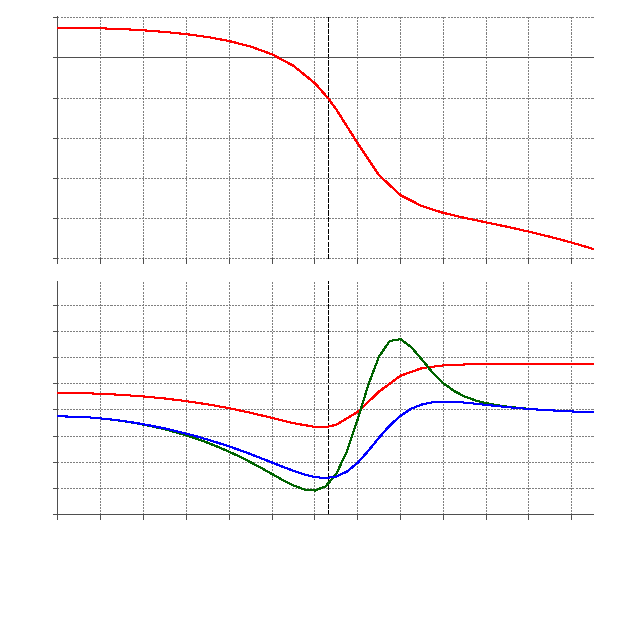
\includegraphics{images/irIsot}}%
    \gplfronttext
  \end{picture}%
\endgroup

  \caption[Isotopic shifts for the different infrared excitations.]
  {Isotopic shifts for the three main different infrared excitations.
  The top panel corresponds to the first infrared-active excitations.
  In the bottom panel the red line corresponds to the excitation with one infrared and one Raman phonon; the green and blue lines to the excitations with two and three infrared phonons respectively.}
  \label{fig:irIsot}
\end{figure}

The first infrared excitation is peculiar since it has a negative isotopic shift for $\lambda > \sim 0.1$ eV with a value of $\sim -5.2$\% for $\lambda_{ir}=0.1263$ eV.
This negative isotopic shift is a signal of polaronic behaviour in the system since harmonic and anharmonic potentials all predict positive isotopic shifts \cite{MustredeLeon2000,Pali1998}.
For large coupling values this isotopic shift remains negative but seems to stabilize near 25\%.
However, there could be some numerical instabilities in this specific isotopic shift attibutable to float-point arithmetic limitations in the calculations since we are dealing with numbers very close to zero\footnote{See https://research-engine.appspot.com/37001/notebooks/2001/4844104634597376 for details.}.

In Table \ref{tab:irIsotShifts} we show the calculated energies for these excitations in the $^{16}$O and $^{18}$O cases as well as the isotopic shift $\Delta_i$ for the $\lambda_{ir}=0.1263$ eV case. It can be seen that all the shifts are smaller than the harmonic prediction. However the strongest deviation is in the eigenstate with one infrared phonon where $\Delta_i$ is negative \cite{GarciaSaraviaOrtizdeMontellano2014}.
 
\begin{table}[ht]
  \centering
  \begin{tabular}[ht]{|l|c|c|c|c|}
    \hline
    Excitation & $\omega_i^{(16)}$ (cm$^{-1}$) & $\omega_i^{(18)}$ (cm$^{-1}$) & $\Delta_i$ (\%) & Harmonic (\%)\\
    \hline
    1 infrared              & 141.39 & 148.56 & -5.07 & 3.75 \\
    1 infrared and 1 Raman  & 641.39 & 619.81 &  3.36 & 4.65 \\
    2 infrared              & 457.60 & 452.25 &  1.17 & 3.75 \\
    3 infrared              & 774.25 & 763.41 &  1.40 & 3.75 \\
    \hline
    \end{tabular}
    \caption[Energies and isotopic shifts for the infrared excitations in the $\lambda_{ir}=0.1263$ eV case.]
    {Energies and isotopic shifts for the three main infrared excitations in the $\lambda_{ir}=0.1263$ eV case compared with the harmonic prediction.}
    \label{tab:irIsotShifts}
\end{table}

\section{Projection into phonon coordinates}
\label{sec:irPhononProj}

As a further visualization of the deviation and recovery of harmonic behaviour with $\lambda_{ir}$ we projected the eigenstates corresponding to two and three infrared phonons into $(u_{ir},u_R)$.
In Figure \ref{fig:phononProj2-3ir} we show a plot of this projection for the three representative coupling values $\lambda_{ir}=0,0.1263$ and 0.25 eV.

\begin{figure}[ht]
  \centering
  % GNUPLOT: LaTeX picture with Postscript
\begingroup
  \makeatletter
  \providecommand\color[2][]{%
    \GenericError{(gnuplot) \space\space\space\@spaces}{%
      Package color not loaded in conjunction with
      terminal option `colourtext'%
    }{See the gnuplot documentation for explanation.%
    }{Either use 'blacktext' in gnuplot or load the package
      color.sty in LaTeX.}%
    \renewcommand\color[2][]{}%
  }%
  \providecommand\includegraphics[2][]{%
    \GenericError{(gnuplot) \space\space\space\@spaces}{%
      Package graphicx or graphics not loaded%
    }{See the gnuplot documentation for explanation.%
    }{The gnuplot epslatex terminal needs graphicx.sty or graphics.sty.}%
    \renewcommand\includegraphics[2][]{}%
  }%
  \providecommand\rotatebox[2]{#2}%
  \@ifundefined{ifGPcolor}{%
    \newif\ifGPcolor
    \GPcolortrue
  }{}%
  \@ifundefined{ifGPblacktext}{%
    \newif\ifGPblacktext
    \GPblacktextfalse
  }{}%
  % define a \g@addto@macro without @ in the name:
  \let\gplgaddtomacro\g@addto@macro
  % define empty templates for all commands taking text:
  \gdef\gplbacktext{}%
  \gdef\gplfronttext{}%
  \makeatother
  \ifGPblacktext
    % no textcolor at all
    \def\colorrgb#1{}%
    \def\colorgray#1{}%
  \else
    % gray or color?
    \ifGPcolor
      \def\colorrgb#1{\color[rgb]{#1}}%
      \def\colorgray#1{\color[gray]{#1}}%
      \expandafter\def\csname LTw\endcsname{\color{white}}%
      \expandafter\def\csname LTb\endcsname{\color{black}}%
      \expandafter\def\csname LTa\endcsname{\color{black}}%
      \expandafter\def\csname LT0\endcsname{\color[rgb]{1,0,0}}%
      \expandafter\def\csname LT1\endcsname{\color[rgb]{0,1,0}}%
      \expandafter\def\csname LT2\endcsname{\color[rgb]{0,0,1}}%
      \expandafter\def\csname LT3\endcsname{\color[rgb]{1,0,1}}%
      \expandafter\def\csname LT4\endcsname{\color[rgb]{0,1,1}}%
      \expandafter\def\csname LT5\endcsname{\color[rgb]{1,1,0}}%
      \expandafter\def\csname LT6\endcsname{\color[rgb]{0,0,0}}%
      \expandafter\def\csname LT7\endcsname{\color[rgb]{1,0.3,0}}%
      \expandafter\def\csname LT8\endcsname{\color[rgb]{0.5,0.5,0.5}}%
    \else
      % gray
      \def\colorrgb#1{\color{black}}%
      \def\colorgray#1{\color[gray]{#1}}%
      \expandafter\def\csname LTw\endcsname{\color{white}}%
      \expandafter\def\csname LTb\endcsname{\color{black}}%
      \expandafter\def\csname LTa\endcsname{\color{black}}%
      \expandafter\def\csname LT0\endcsname{\color{black}}%
      \expandafter\def\csname LT1\endcsname{\color{black}}%
      \expandafter\def\csname LT2\endcsname{\color{black}}%
      \expandafter\def\csname LT3\endcsname{\color{black}}%
      \expandafter\def\csname LT4\endcsname{\color{black}}%
      \expandafter\def\csname LT5\endcsname{\color{black}}%
      \expandafter\def\csname LT6\endcsname{\color{black}}%
      \expandafter\def\csname LT7\endcsname{\color{black}}%
      \expandafter\def\csname LT8\endcsname{\color{black}}%
    \fi
  \fi
  \setlength{\unitlength}{0.0500bp}%
  \begin{picture}(7936.00,4534.00)%
    \gplgaddtomacro\gplbacktext{%
      \csname LTb\endcsname%
      \put(-63,2574){\makebox(0,0)[r]{\strut{}\scriptsize -0.3}}%
      \put(-63,2794){\makebox(0,0)[r]{\strut{}\scriptsize -0.2}}%
      \put(-63,3015){\makebox(0,0)[r]{\strut{}\scriptsize -0.1}}%
      \put(-63,3235){\makebox(0,0)[r]{\strut{}\scriptsize 0}}%
      \put(-63,3455){\makebox(0,0)[r]{\strut{}\scriptsize 0.1}}%
      \put(-63,3676){\makebox(0,0)[r]{\strut{}\scriptsize 0.2}}%
      \put(-63,3896){\makebox(0,0)[r]{\strut{}\scriptsize 0.3}}%
      \put(223,2094){\makebox(0,0){\strut{}\scriptsize -0.4}}%
      \put(799,2094){\makebox(0,0){\strut{}\scriptsize -0.2}}%
      \put(1375,2094){\makebox(0,0){\strut{}\scriptsize 0}}%
      \put(1951,2094){\makebox(0,0){\strut{}\scriptsize 0.2}}%
      \put(2527,2094){\makebox(0,0){\strut{}\scriptsize 0.4}}%
      \put(-569,3235){\rotatebox{-270}{\makebox(0,0){\strut{}$u_{R}$ (\AA)}}}%
      \put(1375,1808){\makebox(0,0){\strut{}}}%
      \put(794,4352){\makebox(0,0)[l]{\strut{}\scriptsize{$\lambda_{ir} = 0.00$ eV}}}%
    }%
    \gplgaddtomacro\gplfronttext{%
    }%
    \gplgaddtomacro\gplbacktext{%
      \csname LTb\endcsname%
      \put(2841,2094){\makebox(0,0){\strut{}\scriptsize -0.4}}%
      \put(3417,2094){\makebox(0,0){\strut{}\scriptsize -0.2}}%
      \put(3994,2094){\makebox(0,0){\strut{}\scriptsize 0}}%
      \put(4570,2094){\makebox(0,0){\strut{}\scriptsize 0.2}}%
      \put(5146,2094){\makebox(0,0){\strut{}\scriptsize 0.4}}%
      \put(3278,3235){\rotatebox{-270}{\makebox(0,0){\strut{}}}}%
      \put(3993,1808){\makebox(0,0){\strut{}}}%
      \put(3412,4352){\makebox(0,0)[l]{\strut{}\scriptsize{$\lambda_{ir} = 0.1263$ eV}}}%
    }%
    \gplgaddtomacro\gplfronttext{%
    }%
    \gplgaddtomacro\gplbacktext{%
      \csname LTb\endcsname%
      \put(5460,2094){\makebox(0,0){\strut{}\scriptsize -0.4}}%
      \put(6036,2094){\makebox(0,0){\strut{}\scriptsize -0.2}}%
      \put(6612,2094){\makebox(0,0){\strut{}\scriptsize 0}}%
      \put(7188,2094){\makebox(0,0){\strut{}\scriptsize 0.2}}%
      \put(7764,2094){\makebox(0,0){\strut{}\scriptsize 0.4}}%
      \put(5897,3235){\rotatebox{-270}{\makebox(0,0){\strut{}}}}%
      \put(6612,1808){\makebox(0,0){\strut{}}}%
      \put(6031,4352){\makebox(0,0)[l]{\strut{}\scriptsize{$\lambda_{ir} = 0.25$ eV}}}%
    }%
    \gplgaddtomacro\gplfronttext{%
    }%
    \gplgaddtomacro\gplbacktext{%
      \csname LTb\endcsname%
      \put(-63,637){\makebox(0,0)[r]{\strut{}\scriptsize -0.3}}%
      \put(-63,858){\makebox(0,0)[r]{\strut{}\scriptsize -0.2}}%
      \put(-63,1078){\makebox(0,0)[r]{\strut{}\scriptsize -0.1}}%
      \put(-63,1299){\makebox(0,0)[r]{\strut{}\scriptsize 0}}%
      \put(-63,1519){\makebox(0,0)[r]{\strut{}\scriptsize 0.1}}%
      \put(-63,1739){\makebox(0,0)[r]{\strut{}\scriptsize 0.2}}%
      \put(-63,1960){\makebox(0,0)[r]{\strut{}\scriptsize 0.3}}%
      \put(223,157){\makebox(0,0){\strut{}\scriptsize -0.4}}%
      \put(799,157){\makebox(0,0){\strut{}\scriptsize -0.2}}%
      \put(1375,157){\makebox(0,0){\strut{}\scriptsize 0}}%
      \put(1951,157){\makebox(0,0){\strut{}\scriptsize 0.2}}%
      \put(2527,157){\makebox(0,0){\strut{}\scriptsize 0.4}}%
      \put(-569,1298){\rotatebox{-270}{\makebox(0,0){\strut{}$u_{R}$ (\AA)}}}%
      \put(1375,-129){\makebox(0,0){\strut{}}}%
      \put(6031,4352){\makebox(0,0)[l]{\strut{}\scriptsize{$\lambda_{ir} = 0.25$ eV}}}%
    }%
    \gplgaddtomacro\gplfronttext{%
    }%
    \gplgaddtomacro\gplbacktext{%
      \csname LTb\endcsname%
      \put(2841,157){\makebox(0,0){\strut{}\scriptsize -0.4}}%
      \put(3417,157){\makebox(0,0){\strut{}\scriptsize -0.2}}%
      \put(3994,157){\makebox(0,0){\strut{}\scriptsize 0}}%
      \put(4570,157){\makebox(0,0){\strut{}\scriptsize 0.2}}%
      \put(5146,157){\makebox(0,0){\strut{}\scriptsize 0.4}}%
      \put(3278,1298){\rotatebox{-270}{\makebox(0,0){\strut{}}}}%
      \put(3993,-173){\makebox(0,0){\strut{}$u_{ir}$ (\AA)}}%
      \put(6031,4352){\makebox(0,0)[l]{\strut{}\scriptsize{$\lambda_{ir} = 0.25$ eV}}}%
    }%
    \gplgaddtomacro\gplfronttext{%
    }%
    \gplgaddtomacro\gplbacktext{%
      \csname LTb\endcsname%
      \put(5460,157){\makebox(0,0){\strut{}\scriptsize -0.4}}%
      \put(6036,157){\makebox(0,0){\strut{}\scriptsize -0.2}}%
      \put(6612,157){\makebox(0,0){\strut{}\scriptsize 0}}%
      \put(7188,157){\makebox(0,0){\strut{}\scriptsize 0.2}}%
      \put(7764,157){\makebox(0,0){\strut{}\scriptsize 0.4}}%
      \put(5897,1298){\rotatebox{-270}{\makebox(0,0){\strut{}}}}%
      \put(6612,-129){\makebox(0,0){\strut{}}}%
      \put(6031,4352){\makebox(0,0)[l]{\strut{}\scriptsize{$\lambda_{ir} = 0.25$ eV}}}%
    }%
    \gplgaddtomacro\gplfronttext{%
    }%
    \gplbacktext
    \put(0,0){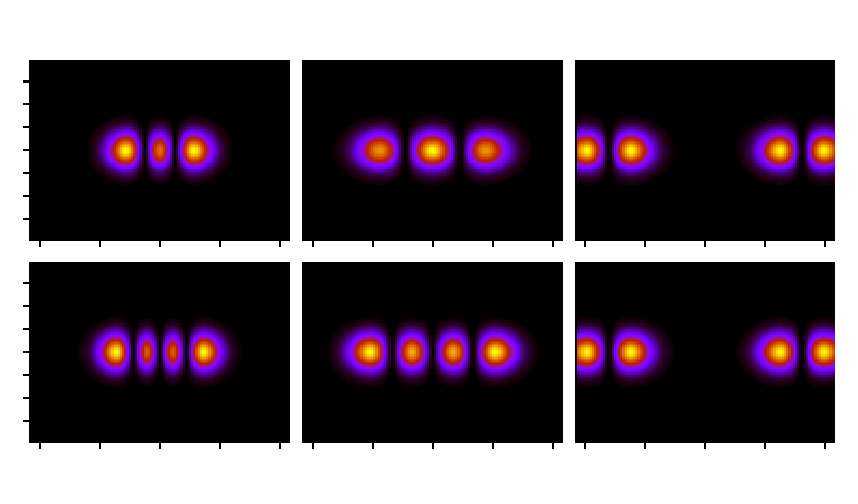
\includegraphics{images/phononProj2-3ir}}%
    \gplfronttext
  \end{picture}%
\endgroup

  \caption[Projection into phonon coordinates of the states with two and three infrared phonons.]
  {Projection into phonon coordinates of the states with two (top) and three (bottom) infrared phonons for three representative $\lambda_{ir}$ values.}
  \label{fig:phononProj2-3ir}
\end{figure}

It is illustrative to compare this plot with Figure \ref{fig:phononProjGrdPol} showing a similar comparison for the ground and first excited states.
In all cases, at $\lambda_{ir}=0$ eV the projection is what can be expected for an harmonic oscillator; it is a simple gaussian when the number of phonons is zero and it has an increasing number of nodes corresponding to the number of phonons in the excitation.
For large $\lambda_{ir}$ the projection of the excitations with two and three infrared phonons become very similar, analogous to the similarity between the ground and first excited states.
It was shown in Figure \ref{fig:irSpectra} that for large $\lambda_{ir}$ the energy of the states with two and three infrared phonons converge to the energy of one infrared phonon, $\omega_{ir}$.
In Figure \ref{fig:phononProj2-3ir} we can see that the projections of these states, for large $\lambda_{ir}$, is similar to two displaced harmonic states with just one infrared phonon.
This is further evidence charge \textit{freezing}, signaling an incipient ferromagnetism, and the distortions in the cluster becoming static.

Since the states with an \textit{even} number of infrared phonons (and an even number of nodes in the $u_{ir}$ projection) converge to states with an \textit{odd} number of infrared phonons (with odd nodes), at some point in the $\lambda_{ir}$ regime they must develop an additional node.
It was shown in \ref{fig:uirCoupl} that, for $\lambda_{ir}=0.1263$ eV, the ground state has already developed a partial peak separation that becomes complete only for $\lambda_{ir}>0.16$ eV.
In contrast the excitation with two infrared phonons, at this same coupling, still has only one central peak that splits at larger coupling values.
